\documentclass{article}
\usepackage{tikz}
\usetikzlibrary{shapes.geometric, arrows}
%\tikzstyle{every state}=[fill=yellow1,draw,text=black]
\tikzstyle{startstop} = [rectangle, rounded corners, 
minimum width=3cm, 
minimum height=2cm,
text centered, 
draw=black]



%  \tikzstyle{every state}=[fill=yellow1,draw,text=black]

\tikzstyle{arrow} = [thick,->,>=stealth]
\begin{document}
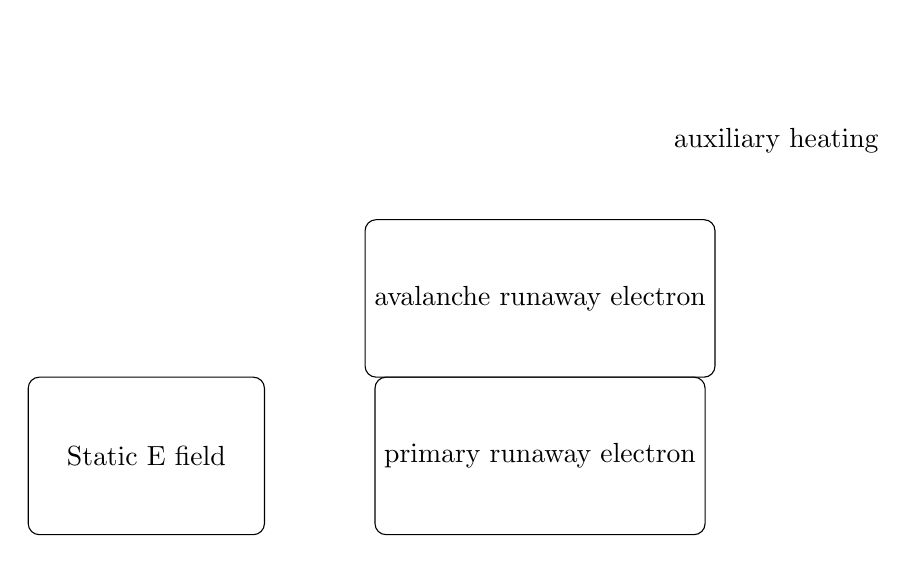
\begin{tikzpicture}[node distance=2cm]
%\node (start) [startstop] {Start};
%\node (in1) [startstop, below of=start] {Input};
\node (E0)[startstop] {Static E field };
\node (pre) [startstop, right of=E0,xshift=3cm] {primary runaway electron};
\node (ave)[startstop,below of =pre,yshift=4cm]{avalanche runaway electron};
\node (ah)[circle,below of =ave,yshift=4cm,xshift=3cm]{auxiliary heating};
%\node(ava)[sbox,below of=pre,yshift=-0.5cm]{RE}
\end{tikzpicture}
\end{document}